\documentclass[twoside]{book}

% Packages required by doxygen
\usepackage{fixltx2e}
\usepackage{calc}
\usepackage{doxygen}
\usepackage[export]{adjustbox} % also loads graphicx
\usepackage{graphicx}
\usepackage[utf8]{inputenc}
\usepackage{makeidx}
\usepackage{multicol}
\usepackage{multirow}
\PassOptionsToPackage{warn}{textcomp}
\usepackage{textcomp}
\usepackage[nointegrals]{wasysym}
\usepackage[table]{xcolor}

% Font selection
\usepackage[T1]{fontenc}
\usepackage[scaled=.90]{helvet}
\usepackage{courier}
\usepackage{amssymb}
\usepackage{sectsty}
\renewcommand{\familydefault}{\sfdefault}
\allsectionsfont{%
  \fontseries{bc}\selectfont%
  \color{darkgray}%
}
\renewcommand{\DoxyLabelFont}{%
  \fontseries{bc}\selectfont%
  \color{darkgray}%
}
\newcommand{\+}{\discretionary{\mbox{\scriptsize$\hookleftarrow$}}{}{}}

% Page & text layout
\usepackage{geometry}
\geometry{%
  a4paper,%
  top=2.5cm,%
  bottom=2.5cm,%
  left=2.5cm,%
  right=2.5cm%
}
\tolerance=750
\hfuzz=15pt
\hbadness=750
\setlength{\emergencystretch}{15pt}
\setlength{\parindent}{0cm}
\setlength{\parskip}{3ex plus 2ex minus 2ex}
\makeatletter
\renewcommand{\paragraph}{%
  \@startsection{paragraph}{4}{0ex}{-1.0ex}{1.0ex}{%
    \normalfont\normalsize\bfseries\SS@parafont%
  }%
}
\renewcommand{\subparagraph}{%
  \@startsection{subparagraph}{5}{0ex}{-1.0ex}{1.0ex}{%
    \normalfont\normalsize\bfseries\SS@subparafont%
  }%
}
\makeatother

% Headers & footers
\usepackage{fancyhdr}
\pagestyle{fancyplain}
\fancyhead[LE]{\fancyplain{}{\bfseries\thepage}}
\fancyhead[CE]{\fancyplain{}{}}
\fancyhead[RE]{\fancyplain{}{\bfseries\leftmark}}
\fancyhead[LO]{\fancyplain{}{\bfseries\rightmark}}
\fancyhead[CO]{\fancyplain{}{}}
\fancyhead[RO]{\fancyplain{}{\bfseries\thepage}}
\fancyfoot[LE]{\fancyplain{}{}}
\fancyfoot[CE]{\fancyplain{}{}}
\fancyfoot[RE]{\fancyplain{}{\bfseries\scriptsize Generated by Doxygen }}
\fancyfoot[LO]{\fancyplain{}{\bfseries\scriptsize Generated by Doxygen }}
\fancyfoot[CO]{\fancyplain{}{}}
\fancyfoot[RO]{\fancyplain{}{}}
\renewcommand{\footrulewidth}{0.4pt}
\renewcommand{\chaptermark}[1]{%
  \markboth{#1}{}%
}
\renewcommand{\sectionmark}[1]{%
  \markright{\thesection\ #1}%
}

% Indices & bibliography
\usepackage{natbib}
\usepackage[titles]{tocloft}
\setcounter{tocdepth}{3}
\setcounter{secnumdepth}{5}
\makeindex

% Hyperlinks (required, but should be loaded last)
\usepackage{ifpdf}
\ifpdf
  \usepackage[pdftex,pagebackref=true]{hyperref}
\else
  \usepackage[ps2pdf,pagebackref=true]{hyperref}
\fi
\hypersetup{%
  colorlinks=true,%
  linkcolor=blue,%
  citecolor=blue,%
  unicode%
}

% Custom commands
\newcommand{\clearemptydoublepage}{%
  \newpage{\pagestyle{empty}\cleardoublepage}%
}

\usepackage{caption}
\captionsetup{labelsep=space,justification=centering,font={bf},singlelinecheck=off,skip=4pt,position=top}

%===== C O N T E N T S =====

\begin{document}

% Titlepage & ToC
\hypersetup{pageanchor=false,
             bookmarksnumbered=true,
             pdfencoding=unicode
            }
\pagenumbering{alph}
\begin{titlepage}
\vspace*{7cm}
\begin{center}%
{\Large Projeto\+\_\+\+Servidor \\[1ex]\large 1.\+0 }\\
\vspace*{1cm}
{\large Generated by Doxygen 1.8.14}\\
\end{center}
\end{titlepage}
\clearemptydoublepage
\pagenumbering{roman}
\tableofcontents
\clearemptydoublepage
\pagenumbering{arabic}
\hypersetup{pageanchor=true}

%--- Begin generated contents ---
\chapter{Namespace Index}
\section{Namespace List}
Here is a list of all namespaces with brief descriptions\+:\begin{DoxyCompactList}
\item\contentsline{section}{\mbox{\hyperlink{namespace_ui}{Ui}} }{\pageref{namespace_ui}}{}
\end{DoxyCompactList}

\chapter{Hierarchical Index}
\section{Class Hierarchy}
This inheritance list is sorted roughly, but not completely, alphabetically\+:\begin{DoxyCompactList}
\item \contentsline{section}{Data\+Storage}{\pageref{class_data_storage}}{}
\item \contentsline{section}{Entry}{\pageref{struct_entry}}{}
\item Q\+Main\+Window\begin{DoxyCompactList}
\item \contentsline{section}{Main\+Window}{\pageref{class_main_window}}{}
\end{DoxyCompactList}
\item \contentsline{section}{qt\+\_\+meta\+\_\+stringdata\+\_\+\+Main\+Window\+\_\+t}{\pageref{structqt__meta__stringdata___main_window__t}}{}
\item \contentsline{section}{qt\+\_\+meta\+\_\+stringdata\+\_\+\+My\+Server\+\_\+t}{\pageref{structqt__meta__stringdata___my_server__t}}{}
\item \contentsline{section}{qt\+\_\+meta\+\_\+stringdata\+\_\+\+My\+Thread\+\_\+t}{\pageref{structqt__meta__stringdata___my_thread__t}}{}
\item Q\+Tcp\+Server\begin{DoxyCompactList}
\item \contentsline{section}{My\+Server}{\pageref{class_my_server}}{}
\end{DoxyCompactList}
\item Q\+Thread\begin{DoxyCompactList}
\item \contentsline{section}{My\+Thread}{\pageref{class_my_thread}}{}
\end{DoxyCompactList}
\item \contentsline{section}{Range\+Test}{\pageref{struct_range_test}}{}
\item \contentsline{section}{Ui\+\_\+\+Main\+Window}{\pageref{class_ui___main_window}}{}
\begin{DoxyCompactList}
\item \contentsline{section}{Ui\+:\+:Main\+Window}{\pageref{class_ui_1_1_main_window}}{}
\end{DoxyCompactList}
\end{DoxyCompactList}

\chapter{Class Index}
\section{Class List}
Here are the classes, structs, unions and interfaces with brief descriptions\+:\begin{DoxyCompactList}
\item\contentsline{section}{\mbox{\hyperlink{class_main_window}{Main\+Window}} \\*The \mbox{\hyperlink{class_main_window}{Main\+Window}} class Classe da janela principal do consumidor de dados }{\pageref{class_main_window}}{}
\item\contentsline{section}{\mbox{\hyperlink{classplotter}{plotter}} \\*The plotter class Classe responsável por representar um gráfico através de um widget }{\pageref{classplotter}}{}
\end{DoxyCompactList}

\chapter{File Index}
\section{File List}
Here is a list of all files with brief descriptions\+:\begin{DoxyCompactList}
\item\contentsline{section}{\mbox{\hyperlink{main_8cpp}{main.\+cpp}} }{\pageref{main_8cpp}}{}
\item\contentsline{section}{\mbox{\hyperlink{mainwindow_8cpp}{mainwindow.\+cpp}} }{\pageref{mainwindow_8cpp}}{}
\item\contentsline{section}{\mbox{\hyperlink{mainwindow_8h}{mainwindow.\+h}} }{\pageref{mainwindow_8h}}{}
\end{DoxyCompactList}

\chapter{Namespace Documentation}
\hypertarget{namespace_ui}{}\section{Ui Namespace Reference}
\label{namespace_ui}\index{Ui@{Ui}}
\subsection*{Classes}
\begin{DoxyCompactItemize}
\item 
class \mbox{\hyperlink{class_ui_1_1_main_window}{Main\+Window}}
\end{DoxyCompactItemize}

\chapter{Class Documentation}
\hypertarget{class_data_storage}{}\section{Data\+Storage Class Reference}
\label{class_data_storage}\index{Data\+Storage@{Data\+Storage}}


{\ttfamily \#include $<$datastorage.\+h$>$}

\subsection*{Public Member Functions}
\begin{DoxyCompactItemize}
\item 
\mbox{\hyperlink{class_data_storage_a22825d40495dae6a5df46d629fb26a3f}{Data\+Storage}} ()
\item 
vector$<$ \mbox{\hyperlink{struct_entry}{Entry}} $>$ \mbox{\hyperlink{class_data_storage_a716fe9bd808cb8ea9f0ef153bf01a633}{get\+Data}} (Q\+Host\+Address address, unsigned int lastn=2)
\item 
void \mbox{\hyperlink{class_data_storage_ab46b18762db5b17b3e0a97150079cb78}{add\+Data}} (Q\+Host\+Address address, qint64 time, float measurement)
\item 
void \mbox{\hyperlink{class_data_storage_a6d1d74566ca198c807a9dbbb16019472}{delete\+Host}} (quint32 address)
\item 
vector$<$ Q\+Host\+Address $>$ \mbox{\hyperlink{class_data_storage_a05e60f4e62fb68f588e3f381d40b6bbd}{get\+Host\+List}} ()
\end{DoxyCompactItemize}


\subsection{Constructor \& Destructor Documentation}
\mbox{\Hypertarget{class_data_storage_a22825d40495dae6a5df46d629fb26a3f}\label{class_data_storage_a22825d40495dae6a5df46d629fb26a3f}} 
\index{Data\+Storage@{Data\+Storage}!Data\+Storage@{Data\+Storage}}
\index{Data\+Storage@{Data\+Storage}!Data\+Storage@{Data\+Storage}}
\subsubsection{\texorpdfstring{Data\+Storage()}{DataStorage()}}
{\footnotesize\ttfamily Data\+Storage\+::\+Data\+Storage (\begin{DoxyParamCaption}{ }\end{DoxyParamCaption})}



\subsection{Member Function Documentation}
\mbox{\Hypertarget{class_data_storage_ab46b18762db5b17b3e0a97150079cb78}\label{class_data_storage_ab46b18762db5b17b3e0a97150079cb78}} 
\index{Data\+Storage@{Data\+Storage}!add\+Data@{add\+Data}}
\index{add\+Data@{add\+Data}!Data\+Storage@{Data\+Storage}}
\subsubsection{\texorpdfstring{add\+Data()}{addData()}}
{\footnotesize\ttfamily void Data\+Storage\+::add\+Data (\begin{DoxyParamCaption}\item[{Q\+Host\+Address}]{address,  }\item[{qint64}]{time,  }\item[{float}]{measurement }\end{DoxyParamCaption})}

\mbox{\Hypertarget{class_data_storage_a6d1d74566ca198c807a9dbbb16019472}\label{class_data_storage_a6d1d74566ca198c807a9dbbb16019472}} 
\index{Data\+Storage@{Data\+Storage}!delete\+Host@{delete\+Host}}
\index{delete\+Host@{delete\+Host}!Data\+Storage@{Data\+Storage}}
\subsubsection{\texorpdfstring{delete\+Host()}{deleteHost()}}
{\footnotesize\ttfamily void Data\+Storage\+::delete\+Host (\begin{DoxyParamCaption}\item[{quint32}]{address }\end{DoxyParamCaption})}

\mbox{\Hypertarget{class_data_storage_a716fe9bd808cb8ea9f0ef153bf01a633}\label{class_data_storage_a716fe9bd808cb8ea9f0ef153bf01a633}} 
\index{Data\+Storage@{Data\+Storage}!get\+Data@{get\+Data}}
\index{get\+Data@{get\+Data}!Data\+Storage@{Data\+Storage}}
\subsubsection{\texorpdfstring{get\+Data()}{getData()}}
{\footnotesize\ttfamily vector$<$ \mbox{\hyperlink{struct_entry}{Entry}} $>$ Data\+Storage\+::get\+Data (\begin{DoxyParamCaption}\item[{Q\+Host\+Address}]{address,  }\item[{unsigned int}]{lastn = {\ttfamily 2} }\end{DoxyParamCaption})}

\mbox{\Hypertarget{class_data_storage_a05e60f4e62fb68f588e3f381d40b6bbd}\label{class_data_storage_a05e60f4e62fb68f588e3f381d40b6bbd}} 
\index{Data\+Storage@{Data\+Storage}!get\+Host\+List@{get\+Host\+List}}
\index{get\+Host\+List@{get\+Host\+List}!Data\+Storage@{Data\+Storage}}
\subsubsection{\texorpdfstring{get\+Host\+List()}{getHostList()}}
{\footnotesize\ttfamily vector$<$ Q\+Host\+Address $>$ Data\+Storage\+::get\+Host\+List (\begin{DoxyParamCaption}{ }\end{DoxyParamCaption})}



The documentation for this class was generated from the following files\+:\begin{DoxyCompactItemize}
\item 
\mbox{\hyperlink{datastorage_8h}{datastorage.\+h}}\item 
\mbox{\hyperlink{datastorage_8cpp}{datastorage.\+cpp}}\end{DoxyCompactItemize}

\hypertarget{struct_entry}{}\section{Entry Struct Reference}
\label{struct_entry}\index{Entry@{Entry}}


{\ttfamily \#include $<$datastorage.\+h$>$}

\subsection*{Public Attributes}
\begin{DoxyCompactItemize}
\item 
qint64 \mbox{\hyperlink{struct_entry_a0a78d616ccc342ef6c34d849288d7c85}{the\+Time}}
\item 
float \mbox{\hyperlink{struct_entry_a78ebc6241b1baaa2551b2cf89f519960}{measurement}}
\end{DoxyCompactItemize}


\subsection{Member Data Documentation}
\mbox{\Hypertarget{struct_entry_a78ebc6241b1baaa2551b2cf89f519960}\label{struct_entry_a78ebc6241b1baaa2551b2cf89f519960}} 
\index{Entry@{Entry}!measurement@{measurement}}
\index{measurement@{measurement}!Entry@{Entry}}
\subsubsection{\texorpdfstring{measurement}{measurement}}
{\footnotesize\ttfamily float Entry\+::measurement}

\mbox{\Hypertarget{struct_entry_a0a78d616ccc342ef6c34d849288d7c85}\label{struct_entry_a0a78d616ccc342ef6c34d849288d7c85}} 
\index{Entry@{Entry}!the\+Time@{the\+Time}}
\index{the\+Time@{the\+Time}!Entry@{Entry}}
\subsubsection{\texorpdfstring{the\+Time}{theTime}}
{\footnotesize\ttfamily qint64 Entry\+::the\+Time}



The documentation for this struct was generated from the following file\+:\begin{DoxyCompactItemize}
\item 
\mbox{\hyperlink{datastorage_8h}{datastorage.\+h}}\end{DoxyCompactItemize}

\hypertarget{class_main_window}{}\section{Main\+Window Class Reference}
\label{class_main_window}\index{Main\+Window@{Main\+Window}}


{\ttfamily \#include $<$mainwindow.\+h$>$}

Inheritance diagram for Main\+Window\+:\begin{figure}[H]
\begin{center}
\leavevmode
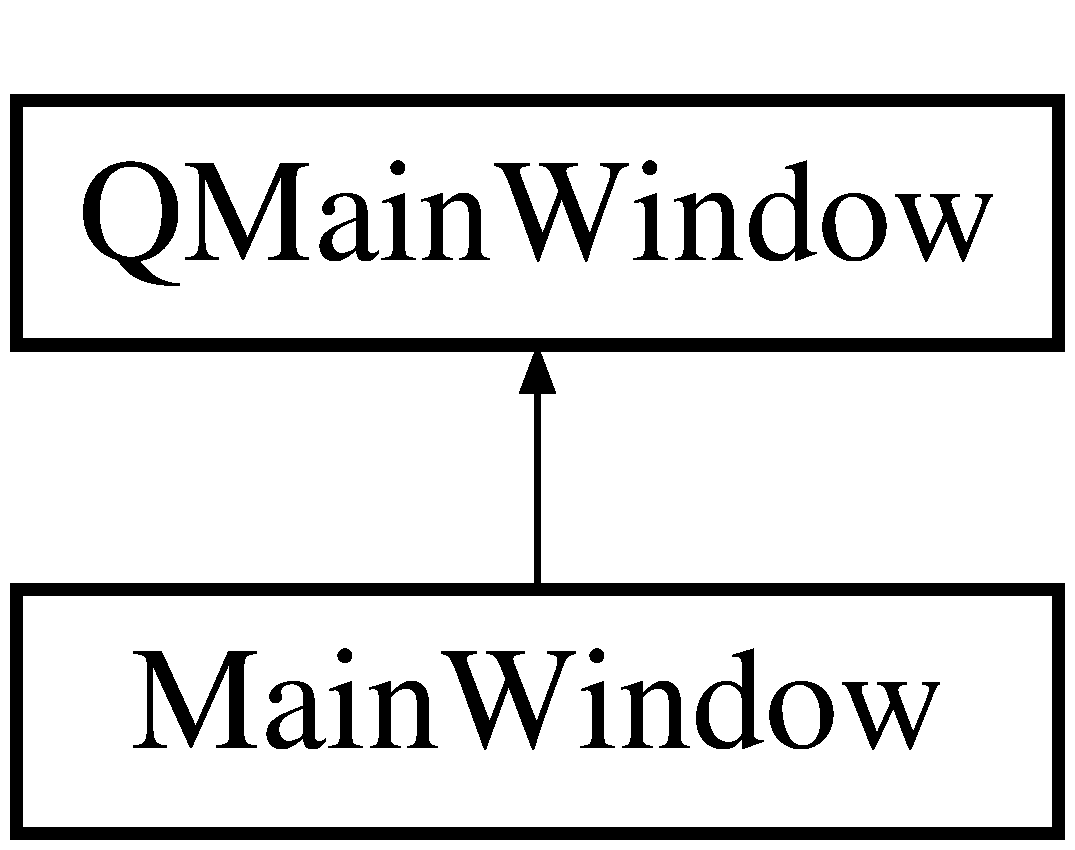
\includegraphics[height=2.000000cm]{class_main_window}
\end{center}
\end{figure}
\subsection*{Public Slots}
\begin{DoxyCompactItemize}
\item 
void \mbox{\hyperlink{class_main_window_a0edca0c59fb238bea02b248c90b89698}{show\+Message}} (Q\+String msg)
\end{DoxyCompactItemize}
\subsection*{Public Member Functions}
\begin{DoxyCompactItemize}
\item 
\mbox{\hyperlink{class_main_window_a8b244be8b7b7db1b08de2a2acb9409db}{Main\+Window}} (Q\+Widget $\ast$parent=0)
\item 
\mbox{\hyperlink{class_main_window_ae98d00a93bc118200eeef9f9bba1dba7}{$\sim$\+Main\+Window}} ()
\end{DoxyCompactItemize}


\subsection{Constructor \& Destructor Documentation}
\mbox{\Hypertarget{class_main_window_a8b244be8b7b7db1b08de2a2acb9409db}\label{class_main_window_a8b244be8b7b7db1b08de2a2acb9409db}} 
\index{Main\+Window@{Main\+Window}!Main\+Window@{Main\+Window}}
\index{Main\+Window@{Main\+Window}!Main\+Window@{Main\+Window}}
\subsubsection{\texorpdfstring{Main\+Window()}{MainWindow()}}
{\footnotesize\ttfamily Main\+Window\+::\+Main\+Window (\begin{DoxyParamCaption}\item[{Q\+Widget $\ast$}]{parent = {\ttfamily 0} }\end{DoxyParamCaption})\hspace{0.3cm}{\ttfamily [explicit]}}

\mbox{\Hypertarget{class_main_window_ae98d00a93bc118200eeef9f9bba1dba7}\label{class_main_window_ae98d00a93bc118200eeef9f9bba1dba7}} 
\index{Main\+Window@{Main\+Window}!````~Main\+Window@{$\sim$\+Main\+Window}}
\index{````~Main\+Window@{$\sim$\+Main\+Window}!Main\+Window@{Main\+Window}}
\subsubsection{\texorpdfstring{$\sim$\+Main\+Window()}{~MainWindow()}}
{\footnotesize\ttfamily Main\+Window\+::$\sim$\+Main\+Window (\begin{DoxyParamCaption}{ }\end{DoxyParamCaption})}



\subsection{Member Function Documentation}
\mbox{\Hypertarget{class_main_window_a0edca0c59fb238bea02b248c90b89698}\label{class_main_window_a0edca0c59fb238bea02b248c90b89698}} 
\index{Main\+Window@{Main\+Window}!show\+Message@{show\+Message}}
\index{show\+Message@{show\+Message}!Main\+Window@{Main\+Window}}
\subsubsection{\texorpdfstring{show\+Message}{showMessage}}
{\footnotesize\ttfamily void Main\+Window\+::show\+Message (\begin{DoxyParamCaption}\item[{Q\+String}]{msg }\end{DoxyParamCaption})\hspace{0.3cm}{\ttfamily [slot]}}



The documentation for this class was generated from the following files\+:\begin{DoxyCompactItemize}
\item 
\mbox{\hyperlink{mainwindow_8h}{mainwindow.\+h}}\item 
\mbox{\hyperlink{mainwindow_8cpp}{mainwindow.\+cpp}}\end{DoxyCompactItemize}

\hypertarget{class_ui_1_1_main_window}{}\section{Ui\+:\+:Main\+Window Class Reference}
\label{class_ui_1_1_main_window}\index{Ui\+::\+Main\+Window@{Ui\+::\+Main\+Window}}


{\ttfamily \#include $<$ui\+\_\+mainwindow.\+h$>$}

Inheritance diagram for Ui\+:\+:Main\+Window\+:\begin{figure}[H]
\begin{center}
\leavevmode
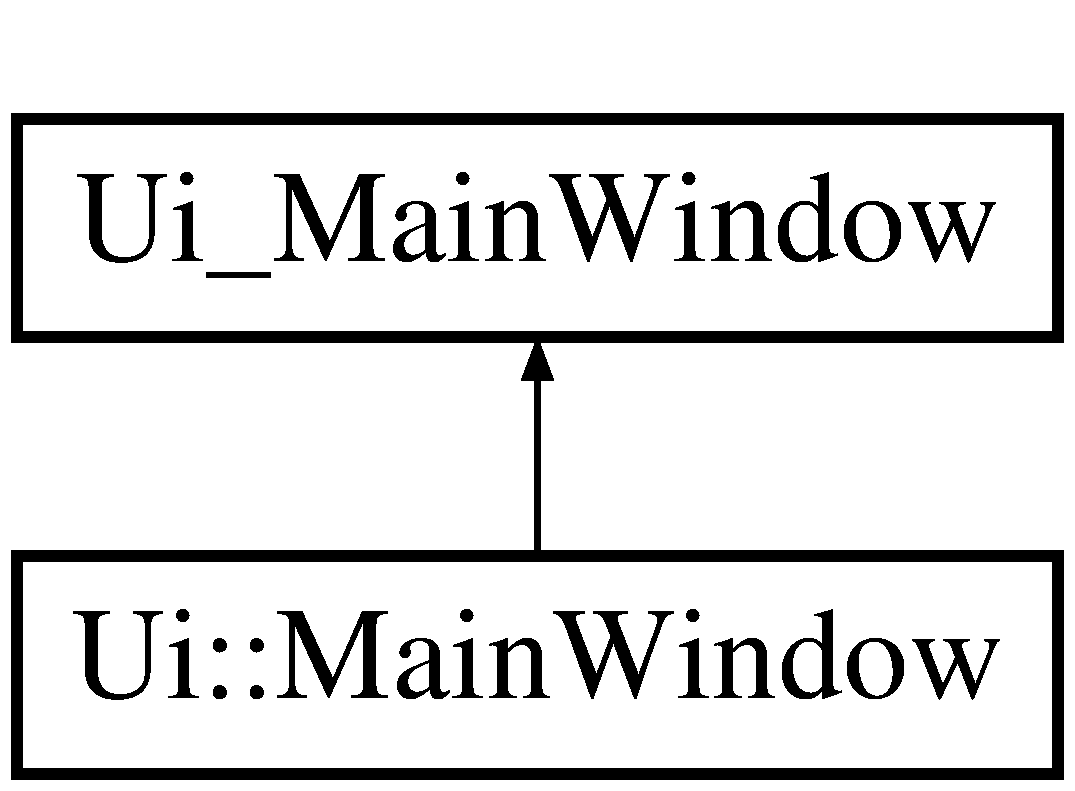
\includegraphics[height=2.000000cm]{class_ui_1_1_main_window}
\end{center}
\end{figure}
\subsection*{Additional Inherited Members}


The documentation for this class was generated from the following file\+:\begin{DoxyCompactItemize}
\item 
\mbox{\hyperlink{ui__mainwindow_8h}{ui\+\_\+mainwindow.\+h}}\end{DoxyCompactItemize}

\hypertarget{class_my_server}{}\section{My\+Server Class Reference}
\label{class_my_server}\index{My\+Server@{My\+Server}}


The \mbox{\hyperlink{class_my_server}{My\+Server}} class inicia um servidor T\+CP capaz de \char`\"{}ouvir\char`\"{} a porta 1234.  




{\ttfamily \#include $<$myserver.\+h$>$}

Inheritance diagram for My\+Server\+:\begin{figure}[H]
\begin{center}
\leavevmode
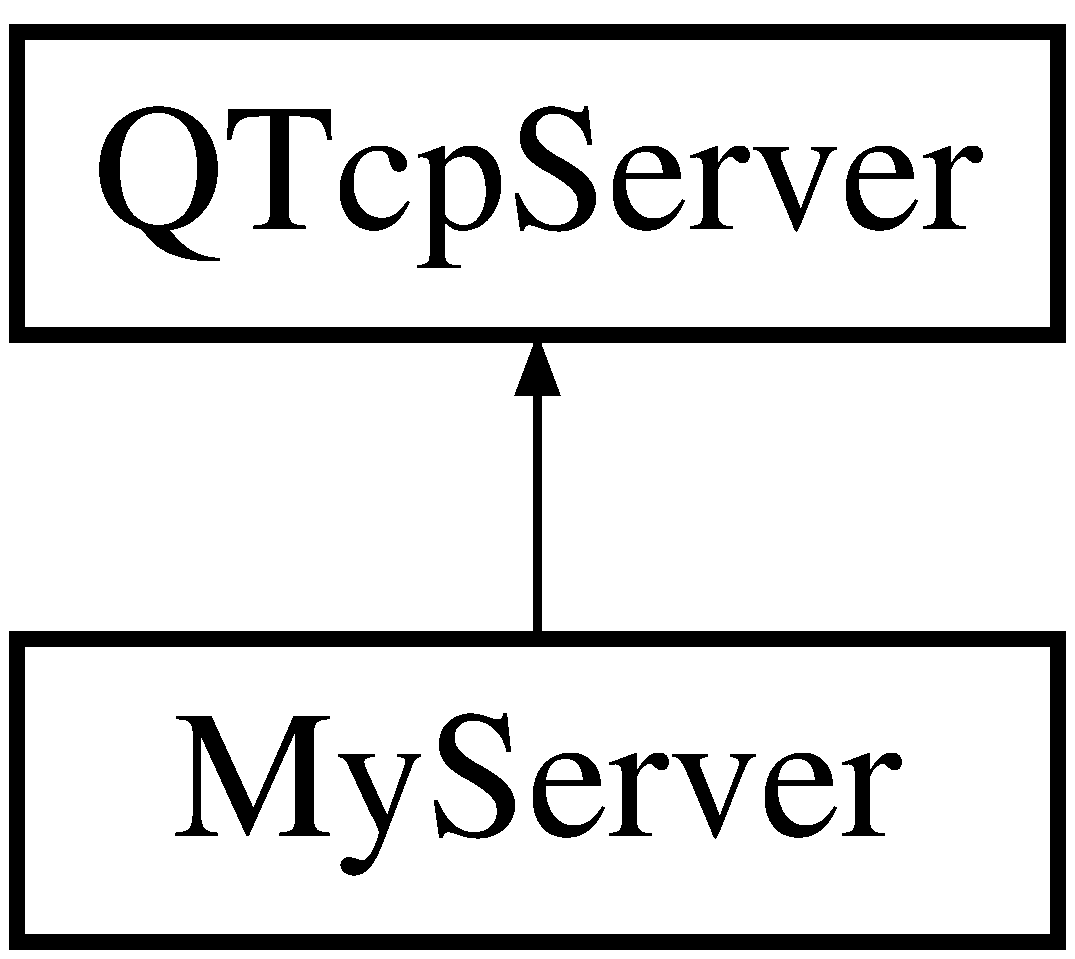
\includegraphics[height=2.000000cm]{class_my_server}
\end{center}
\end{figure}
\subsection*{Public Slots}
\begin{DoxyCompactItemize}
\item 
void \mbox{\hyperlink{class_my_server_ac795ee6f1607c0fa4e635a0da2bf2164}{receive\+Msg}} (Q\+String str)
\end{DoxyCompactItemize}
\subsection*{Signals}
\begin{DoxyCompactItemize}
\item 
void \mbox{\hyperlink{class_my_server_a2b884bce37840b1b461363a37b463b30}{message}} (Q\+String)
\end{DoxyCompactItemize}
\subsection*{Public Member Functions}
\begin{DoxyCompactItemize}
\item 
\mbox{\hyperlink{class_my_server_ac9e5ca7b551a5df90d5b39260f7e5404}{My\+Server}} (Q\+Object $\ast$parent=0)
\begin{DoxyCompactList}\small\item\em \mbox{\hyperlink{class_my_server}{My\+Server}} é o construtor da classe. \end{DoxyCompactList}\item 
void \mbox{\hyperlink{class_my_server_a962f0e205a0aaf08b12d50d1315a8c90}{start\+Server}} ()
\begin{DoxyCompactList}\small\item\em Start\+Server start the T\+CP server. \end{DoxyCompactList}\item 
Q\+String\+List \mbox{\hyperlink{class_my_server_ac10d498dcc2b5d691f131f17b6602a59}{get\+I\+P\+List}} ()
\begin{DoxyCompactList}\small\item\em get\+I\+P\+List return a list of I\+Ps used by server \end{DoxyCompactList}\end{DoxyCompactItemize}
\subsection*{Protected Member Functions}
\begin{DoxyCompactItemize}
\item 
void \mbox{\hyperlink{class_my_server_a635c7a1e6817285ffb1a2a3842df010b}{incoming\+Connection}} (qintptr socket\+Descriptor)
\begin{DoxyCompactList}\small\item\em incoming\+Connection decide o que fazer quando uma nova conexao é iniciada \end{DoxyCompactList}\end{DoxyCompactItemize}


\subsection{Detailed Description}
The \mbox{\hyperlink{class_my_server}{My\+Server}} class inicia um servidor T\+CP capaz de \char`\"{}ouvir\char`\"{} a porta 1234. 

\subsection{Constructor \& Destructor Documentation}
\mbox{\Hypertarget{class_my_server_ac9e5ca7b551a5df90d5b39260f7e5404}\label{class_my_server_ac9e5ca7b551a5df90d5b39260f7e5404}} 
\index{My\+Server@{My\+Server}!My\+Server@{My\+Server}}
\index{My\+Server@{My\+Server}!My\+Server@{My\+Server}}
\subsubsection{\texorpdfstring{My\+Server()}{MyServer()}}
{\footnotesize\ttfamily My\+Server\+::\+My\+Server (\begin{DoxyParamCaption}\item[{Q\+Object $\ast$}]{parent = {\ttfamily 0} }\end{DoxyParamCaption})}



\mbox{\hyperlink{class_my_server}{My\+Server}} é o construtor da classe. 


\begin{DoxyParams}{Parameters}
{\em parent} & eh o pai do objeto (nao usado) \\
\hline
\end{DoxyParams}


\subsection{Member Function Documentation}
\mbox{\Hypertarget{class_my_server_ac10d498dcc2b5d691f131f17b6602a59}\label{class_my_server_ac10d498dcc2b5d691f131f17b6602a59}} 
\index{My\+Server@{My\+Server}!get\+I\+P\+List@{get\+I\+P\+List}}
\index{get\+I\+P\+List@{get\+I\+P\+List}!My\+Server@{My\+Server}}
\subsubsection{\texorpdfstring{get\+I\+P\+List()}{getIPList()}}
{\footnotesize\ttfamily Q\+String\+List My\+Server\+::get\+I\+P\+List (\begin{DoxyParamCaption}{ }\end{DoxyParamCaption})}



get\+I\+P\+List return a list of I\+Ps used by server 

\begin{DoxyReturn}{Returns}

\end{DoxyReturn}
\mbox{\Hypertarget{class_my_server_a635c7a1e6817285ffb1a2a3842df010b}\label{class_my_server_a635c7a1e6817285ffb1a2a3842df010b}} 
\index{My\+Server@{My\+Server}!incoming\+Connection@{incoming\+Connection}}
\index{incoming\+Connection@{incoming\+Connection}!My\+Server@{My\+Server}}
\subsubsection{\texorpdfstring{incoming\+Connection()}{incomingConnection()}}
{\footnotesize\ttfamily void My\+Server\+::incoming\+Connection (\begin{DoxyParamCaption}\item[{qintptr}]{socket\+Descriptor }\end{DoxyParamCaption})\hspace{0.3cm}{\ttfamily [protected]}}



incoming\+Connection decide o que fazer quando uma nova conexao é iniciada 


\begin{DoxyParams}{Parameters}
{\em socket\+Descriptor} & é o identificador do socket para a conexao \\
\hline
\end{DoxyParams}
\mbox{\Hypertarget{class_my_server_a2b884bce37840b1b461363a37b463b30}\label{class_my_server_a2b884bce37840b1b461363a37b463b30}} 
\index{My\+Server@{My\+Server}!message@{message}}
\index{message@{message}!My\+Server@{My\+Server}}
\subsubsection{\texorpdfstring{message}{message}}
{\footnotesize\ttfamily void My\+Server\+::message (\begin{DoxyParamCaption}\item[{Q\+String}]{\+\_\+t1 }\end{DoxyParamCaption})\hspace{0.3cm}{\ttfamily [signal]}}

\mbox{\Hypertarget{class_my_server_ac795ee6f1607c0fa4e635a0da2bf2164}\label{class_my_server_ac795ee6f1607c0fa4e635a0da2bf2164}} 
\index{My\+Server@{My\+Server}!receive\+Msg@{receive\+Msg}}
\index{receive\+Msg@{receive\+Msg}!My\+Server@{My\+Server}}
\subsubsection{\texorpdfstring{receive\+Msg}{receiveMsg}}
{\footnotesize\ttfamily void My\+Server\+::receive\+Msg (\begin{DoxyParamCaption}\item[{Q\+String}]{str }\end{DoxyParamCaption})\hspace{0.3cm}{\ttfamily [slot]}}

\mbox{\Hypertarget{class_my_server_a962f0e205a0aaf08b12d50d1315a8c90}\label{class_my_server_a962f0e205a0aaf08b12d50d1315a8c90}} 
\index{My\+Server@{My\+Server}!start\+Server@{start\+Server}}
\index{start\+Server@{start\+Server}!My\+Server@{My\+Server}}
\subsubsection{\texorpdfstring{start\+Server()}{startServer()}}
{\footnotesize\ttfamily void My\+Server\+::start\+Server (\begin{DoxyParamCaption}{ }\end{DoxyParamCaption})}



Start\+Server start the T\+CP server. 



The documentation for this class was generated from the following files\+:\begin{DoxyCompactItemize}
\item 
\mbox{\hyperlink{myserver_8h}{myserver.\+h}}\item 
\mbox{\hyperlink{moc__myserver_8cpp}{moc\+\_\+myserver.\+cpp}}\item 
\mbox{\hyperlink{myserver_8cpp}{myserver.\+cpp}}\end{DoxyCompactItemize}

\hypertarget{class_my_thread}{}\section{My\+Thread Class Reference}
\label{class_my_thread}\index{My\+Thread@{My\+Thread}}


The \mbox{\hyperlink{class_my_thread}{My\+Thread}} class cria uma thread que lida com o tratamento de uma conexao T\+CP de entrada.  




{\ttfamily \#include $<$mythread.\+h$>$}

Inheritance diagram for My\+Thread\+:\begin{figure}[H]
\begin{center}
\leavevmode
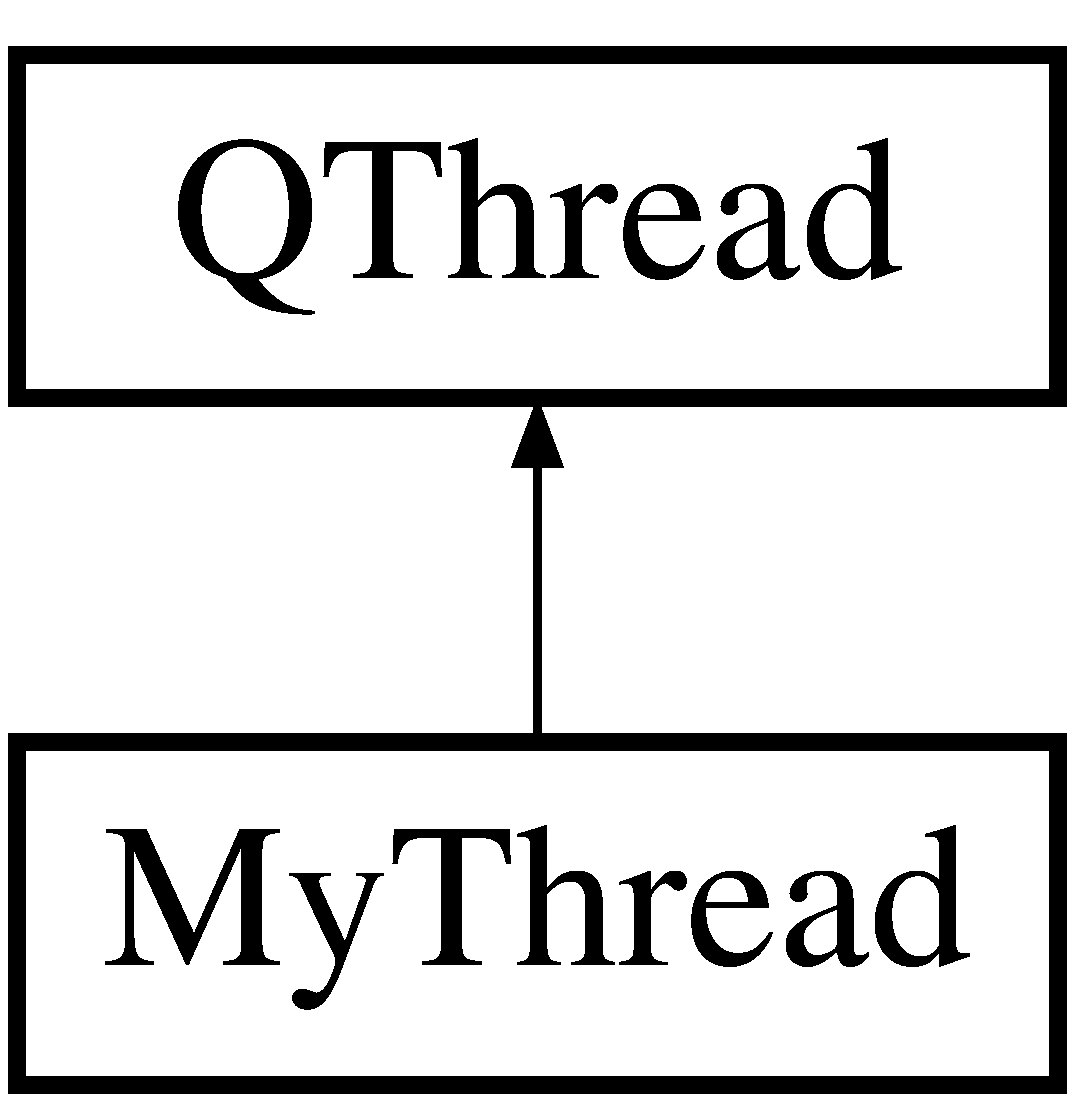
\includegraphics[height=2.000000cm]{class_my_thread}
\end{center}
\end{figure}
\subsection*{Public Slots}
\begin{DoxyCompactItemize}
\item 
void \mbox{\hyperlink{class_my_thread_a277618fdd448b927f2e250c2076fc176}{ready\+Read}} ()
\item 
void \mbox{\hyperlink{class_my_thread_a447710039787ae20134a9b572487840f}{disconnected}} ()
\end{DoxyCompactItemize}
\subsection*{Signals}
\begin{DoxyCompactItemize}
\item 
void \mbox{\hyperlink{class_my_thread_aebf11d93838f22c9547d0c6aa97002be}{error}} (Q\+Tcp\+Socket\+::\+Socket\+Error socketerror)
\item 
void \mbox{\hyperlink{class_my_thread_ae49528d4ec1b2208240f707f5aa74adf}{message}} (Q\+String)
\end{DoxyCompactItemize}
\subsection*{Public Member Functions}
\begin{DoxyCompactItemize}
\item 
\mbox{\hyperlink{class_my_thread_ac1b04b0fa6b32038e810c7105ef762f6}{My\+Thread}} (int ID, Q\+Object $\ast$parent, \mbox{\hyperlink{class_data_storage}{Data\+Storage}} $\ast$storage)
\begin{DoxyCompactList}\small\item\em \mbox{\hyperlink{class_my_thread}{My\+Thread}} eh o construtor da classe. \end{DoxyCompactList}\item 
void \mbox{\hyperlink{class_my_thread_a48f2e366e852087c53705f64e1ee65c2}{run}} ()
\end{DoxyCompactItemize}


\subsection{Detailed Description}
The \mbox{\hyperlink{class_my_thread}{My\+Thread}} class cria uma thread que lida com o tratamento de uma conexao T\+CP de entrada. 

\subsection{Constructor \& Destructor Documentation}
\mbox{\Hypertarget{class_my_thread_ac1b04b0fa6b32038e810c7105ef762f6}\label{class_my_thread_ac1b04b0fa6b32038e810c7105ef762f6}} 
\index{My\+Thread@{My\+Thread}!My\+Thread@{My\+Thread}}
\index{My\+Thread@{My\+Thread}!My\+Thread@{My\+Thread}}
\subsubsection{\texorpdfstring{My\+Thread()}{MyThread()}}
{\footnotesize\ttfamily My\+Thread\+::\+My\+Thread (\begin{DoxyParamCaption}\item[{int}]{ID,  }\item[{Q\+Object $\ast$}]{parent,  }\item[{\mbox{\hyperlink{class_data_storage}{Data\+Storage}} $\ast$}]{storage }\end{DoxyParamCaption})}



\mbox{\hyperlink{class_my_thread}{My\+Thread}} eh o construtor da classe. 


\begin{DoxyParams}{Parameters}
{\em ID} & eh o identificador da thread \\
\hline
{\em parent} & \\
\hline
{\em storage} & \\
\hline
\end{DoxyParams}


\subsection{Member Function Documentation}
\mbox{\Hypertarget{class_my_thread_a447710039787ae20134a9b572487840f}\label{class_my_thread_a447710039787ae20134a9b572487840f}} 
\index{My\+Thread@{My\+Thread}!disconnected@{disconnected}}
\index{disconnected@{disconnected}!My\+Thread@{My\+Thread}}
\subsubsection{\texorpdfstring{disconnected}{disconnected}}
{\footnotesize\ttfamily void My\+Thread\+::disconnected (\begin{DoxyParamCaption}{ }\end{DoxyParamCaption})\hspace{0.3cm}{\ttfamily [slot]}}

\mbox{\Hypertarget{class_my_thread_aebf11d93838f22c9547d0c6aa97002be}\label{class_my_thread_aebf11d93838f22c9547d0c6aa97002be}} 
\index{My\+Thread@{My\+Thread}!error@{error}}
\index{error@{error}!My\+Thread@{My\+Thread}}
\subsubsection{\texorpdfstring{error}{error}}
{\footnotesize\ttfamily void My\+Thread\+::error (\begin{DoxyParamCaption}\item[{Q\+Tcp\+Socket\+::\+Socket\+Error}]{socketerror }\end{DoxyParamCaption})\hspace{0.3cm}{\ttfamily [signal]}}

\mbox{\Hypertarget{class_my_thread_ae49528d4ec1b2208240f707f5aa74adf}\label{class_my_thread_ae49528d4ec1b2208240f707f5aa74adf}} 
\index{My\+Thread@{My\+Thread}!message@{message}}
\index{message@{message}!My\+Thread@{My\+Thread}}
\subsubsection{\texorpdfstring{message}{message}}
{\footnotesize\ttfamily void My\+Thread\+::message (\begin{DoxyParamCaption}\item[{Q\+String}]{\+\_\+t1 }\end{DoxyParamCaption})\hspace{0.3cm}{\ttfamily [signal]}}

\mbox{\Hypertarget{class_my_thread_a277618fdd448b927f2e250c2076fc176}\label{class_my_thread_a277618fdd448b927f2e250c2076fc176}} 
\index{My\+Thread@{My\+Thread}!ready\+Read@{ready\+Read}}
\index{ready\+Read@{ready\+Read}!My\+Thread@{My\+Thread}}
\subsubsection{\texorpdfstring{ready\+Read}{readyRead}}
{\footnotesize\ttfamily void My\+Thread\+::ready\+Read (\begin{DoxyParamCaption}{ }\end{DoxyParamCaption})\hspace{0.3cm}{\ttfamily [slot]}}

\mbox{\Hypertarget{class_my_thread_a48f2e366e852087c53705f64e1ee65c2}\label{class_my_thread_a48f2e366e852087c53705f64e1ee65c2}} 
\index{My\+Thread@{My\+Thread}!run@{run}}
\index{run@{run}!My\+Thread@{My\+Thread}}
\subsubsection{\texorpdfstring{run()}{run()}}
{\footnotesize\ttfamily void My\+Thread\+::run (\begin{DoxyParamCaption}{ }\end{DoxyParamCaption})}



The documentation for this class was generated from the following files\+:\begin{DoxyCompactItemize}
\item 
\mbox{\hyperlink{mythread_8h}{mythread.\+h}}\item 
\mbox{\hyperlink{moc__mythread_8cpp}{moc\+\_\+mythread.\+cpp}}\item 
\mbox{\hyperlink{mythread_8cpp}{mythread.\+cpp}}\end{DoxyCompactItemize}

\hypertarget{structqt__meta__stringdata___main_window__t}{}\section{qt\+\_\+meta\+\_\+stringdata\+\_\+\+Main\+Window\+\_\+t Struct Reference}
\label{structqt__meta__stringdata___main_window__t}\index{qt\+\_\+meta\+\_\+stringdata\+\_\+\+Main\+Window\+\_\+t@{qt\+\_\+meta\+\_\+stringdata\+\_\+\+Main\+Window\+\_\+t}}
\subsection*{Public Attributes}
\begin{DoxyCompactItemize}
\item 
Q\+Byte\+Array\+Data \mbox{\hyperlink{structqt__meta__stringdata___main_window__t_a332d7fa058028f7613b5ba68abb5a7fe}{data}} \mbox{[}4\mbox{]}
\item 
char \mbox{\hyperlink{structqt__meta__stringdata___main_window__t_a10e266ffded4c5e956d35d922fa94828}{stringdata0}} \mbox{[}28\mbox{]}
\end{DoxyCompactItemize}


\subsection{Member Data Documentation}
\mbox{\Hypertarget{structqt__meta__stringdata___main_window__t_a332d7fa058028f7613b5ba68abb5a7fe}\label{structqt__meta__stringdata___main_window__t_a332d7fa058028f7613b5ba68abb5a7fe}} 
\index{qt\+\_\+meta\+\_\+stringdata\+\_\+\+Main\+Window\+\_\+t@{qt\+\_\+meta\+\_\+stringdata\+\_\+\+Main\+Window\+\_\+t}!data@{data}}
\index{data@{data}!qt\+\_\+meta\+\_\+stringdata\+\_\+\+Main\+Window\+\_\+t@{qt\+\_\+meta\+\_\+stringdata\+\_\+\+Main\+Window\+\_\+t}}
\subsubsection{\texorpdfstring{data}{data}}
{\footnotesize\ttfamily Q\+Byte\+Array\+Data qt\+\_\+meta\+\_\+stringdata\+\_\+\+Main\+Window\+\_\+t\+::data\mbox{[}4\mbox{]}}

\mbox{\Hypertarget{structqt__meta__stringdata___main_window__t_a10e266ffded4c5e956d35d922fa94828}\label{structqt__meta__stringdata___main_window__t_a10e266ffded4c5e956d35d922fa94828}} 
\index{qt\+\_\+meta\+\_\+stringdata\+\_\+\+Main\+Window\+\_\+t@{qt\+\_\+meta\+\_\+stringdata\+\_\+\+Main\+Window\+\_\+t}!stringdata0@{stringdata0}}
\index{stringdata0@{stringdata0}!qt\+\_\+meta\+\_\+stringdata\+\_\+\+Main\+Window\+\_\+t@{qt\+\_\+meta\+\_\+stringdata\+\_\+\+Main\+Window\+\_\+t}}
\subsubsection{\texorpdfstring{stringdata0}{stringdata0}}
{\footnotesize\ttfamily char qt\+\_\+meta\+\_\+stringdata\+\_\+\+Main\+Window\+\_\+t\+::stringdata0\mbox{[}28\mbox{]}}



The documentation for this struct was generated from the following file\+:\begin{DoxyCompactItemize}
\item 
\mbox{\hyperlink{moc__mainwindow_8cpp}{moc\+\_\+mainwindow.\+cpp}}\end{DoxyCompactItemize}

\hypertarget{structqt__meta__stringdata___my_server__t}{}\section{qt\+\_\+meta\+\_\+stringdata\+\_\+\+My\+Server\+\_\+t Struct Reference}
\label{structqt__meta__stringdata___my_server__t}\index{qt\+\_\+meta\+\_\+stringdata\+\_\+\+My\+Server\+\_\+t@{qt\+\_\+meta\+\_\+stringdata\+\_\+\+My\+Server\+\_\+t}}
\subsection*{Public Attributes}
\begin{DoxyCompactItemize}
\item 
Q\+Byte\+Array\+Data \mbox{\hyperlink{structqt__meta__stringdata___my_server__t_ab15722048201cc80be7f2b05eece64e9}{data}} \mbox{[}5\mbox{]}
\item 
char \mbox{\hyperlink{structqt__meta__stringdata___my_server__t_a54652770c5771b1f6db92acb7932b3dd}{stringdata0}} \mbox{[}33\mbox{]}
\end{DoxyCompactItemize}


\subsection{Member Data Documentation}
\mbox{\Hypertarget{structqt__meta__stringdata___my_server__t_ab15722048201cc80be7f2b05eece64e9}\label{structqt__meta__stringdata___my_server__t_ab15722048201cc80be7f2b05eece64e9}} 
\index{qt\+\_\+meta\+\_\+stringdata\+\_\+\+My\+Server\+\_\+t@{qt\+\_\+meta\+\_\+stringdata\+\_\+\+My\+Server\+\_\+t}!data@{data}}
\index{data@{data}!qt\+\_\+meta\+\_\+stringdata\+\_\+\+My\+Server\+\_\+t@{qt\+\_\+meta\+\_\+stringdata\+\_\+\+My\+Server\+\_\+t}}
\subsubsection{\texorpdfstring{data}{data}}
{\footnotesize\ttfamily Q\+Byte\+Array\+Data qt\+\_\+meta\+\_\+stringdata\+\_\+\+My\+Server\+\_\+t\+::data\mbox{[}5\mbox{]}}

\mbox{\Hypertarget{structqt__meta__stringdata___my_server__t_a54652770c5771b1f6db92acb7932b3dd}\label{structqt__meta__stringdata___my_server__t_a54652770c5771b1f6db92acb7932b3dd}} 
\index{qt\+\_\+meta\+\_\+stringdata\+\_\+\+My\+Server\+\_\+t@{qt\+\_\+meta\+\_\+stringdata\+\_\+\+My\+Server\+\_\+t}!stringdata0@{stringdata0}}
\index{stringdata0@{stringdata0}!qt\+\_\+meta\+\_\+stringdata\+\_\+\+My\+Server\+\_\+t@{qt\+\_\+meta\+\_\+stringdata\+\_\+\+My\+Server\+\_\+t}}
\subsubsection{\texorpdfstring{stringdata0}{stringdata0}}
{\footnotesize\ttfamily char qt\+\_\+meta\+\_\+stringdata\+\_\+\+My\+Server\+\_\+t\+::stringdata0\mbox{[}33\mbox{]}}



The documentation for this struct was generated from the following file\+:\begin{DoxyCompactItemize}
\item 
\mbox{\hyperlink{moc__myserver_8cpp}{moc\+\_\+myserver.\+cpp}}\end{DoxyCompactItemize}

\hypertarget{structqt__meta__stringdata___my_thread__t}{}\section{qt\+\_\+meta\+\_\+stringdata\+\_\+\+My\+Thread\+\_\+t Struct Reference}
\label{structqt__meta__stringdata___my_thread__t}\index{qt\+\_\+meta\+\_\+stringdata\+\_\+\+My\+Thread\+\_\+t@{qt\+\_\+meta\+\_\+stringdata\+\_\+\+My\+Thread\+\_\+t}}
\subsection*{Public Attributes}
\begin{DoxyCompactItemize}
\item 
Q\+Byte\+Array\+Data \mbox{\hyperlink{structqt__meta__stringdata___my_thread__t_ab5607f1078333a9d42458336e4f735dd}{data}} \mbox{[}8\mbox{]}
\item 
char \mbox{\hyperlink{structqt__meta__stringdata___my_thread__t_aa80f739ca8c1b5cfcf28f7f8d8666688}{stringdata0}} \mbox{[}83\mbox{]}
\end{DoxyCompactItemize}


\subsection{Member Data Documentation}
\mbox{\Hypertarget{structqt__meta__stringdata___my_thread__t_ab5607f1078333a9d42458336e4f735dd}\label{structqt__meta__stringdata___my_thread__t_ab5607f1078333a9d42458336e4f735dd}} 
\index{qt\+\_\+meta\+\_\+stringdata\+\_\+\+My\+Thread\+\_\+t@{qt\+\_\+meta\+\_\+stringdata\+\_\+\+My\+Thread\+\_\+t}!data@{data}}
\index{data@{data}!qt\+\_\+meta\+\_\+stringdata\+\_\+\+My\+Thread\+\_\+t@{qt\+\_\+meta\+\_\+stringdata\+\_\+\+My\+Thread\+\_\+t}}
\subsubsection{\texorpdfstring{data}{data}}
{\footnotesize\ttfamily Q\+Byte\+Array\+Data qt\+\_\+meta\+\_\+stringdata\+\_\+\+My\+Thread\+\_\+t\+::data\mbox{[}8\mbox{]}}

\mbox{\Hypertarget{structqt__meta__stringdata___my_thread__t_aa80f739ca8c1b5cfcf28f7f8d8666688}\label{structqt__meta__stringdata___my_thread__t_aa80f739ca8c1b5cfcf28f7f8d8666688}} 
\index{qt\+\_\+meta\+\_\+stringdata\+\_\+\+My\+Thread\+\_\+t@{qt\+\_\+meta\+\_\+stringdata\+\_\+\+My\+Thread\+\_\+t}!stringdata0@{stringdata0}}
\index{stringdata0@{stringdata0}!qt\+\_\+meta\+\_\+stringdata\+\_\+\+My\+Thread\+\_\+t@{qt\+\_\+meta\+\_\+stringdata\+\_\+\+My\+Thread\+\_\+t}}
\subsubsection{\texorpdfstring{stringdata0}{stringdata0}}
{\footnotesize\ttfamily char qt\+\_\+meta\+\_\+stringdata\+\_\+\+My\+Thread\+\_\+t\+::stringdata0\mbox{[}83\mbox{]}}



The documentation for this struct was generated from the following file\+:\begin{DoxyCompactItemize}
\item 
\mbox{\hyperlink{moc__mythread_8cpp}{moc\+\_\+mythread.\+cpp}}\end{DoxyCompactItemize}

\hypertarget{struct_range_test}{}\section{Range\+Test Struct Reference}
\label{struct_range_test}\index{Range\+Test@{Range\+Test}}
\subsection*{Public Member Functions}
\begin{DoxyCompactItemize}
\item 
\mbox{\hyperlink{struct_range_test_a9d96f82c111ffd4d2747416b90306791}{Range\+Test}} (qint64 \+\_\+limit)
\item 
bool \mbox{\hyperlink{struct_range_test_add496768a566e04219e840ee25e829d7}{operator()}} (qint64 n)
\end{DoxyCompactItemize}
\subsection*{Public Attributes}
\begin{DoxyCompactItemize}
\item 
qint64 \mbox{\hyperlink{struct_range_test_a638ebd61c0447db219f10cd1473ab364}{limit}}
\end{DoxyCompactItemize}


\subsection{Constructor \& Destructor Documentation}
\mbox{\Hypertarget{struct_range_test_a9d96f82c111ffd4d2747416b90306791}\label{struct_range_test_a9d96f82c111ffd4d2747416b90306791}} 
\index{Range\+Test@{Range\+Test}!Range\+Test@{Range\+Test}}
\index{Range\+Test@{Range\+Test}!Range\+Test@{Range\+Test}}
\subsubsection{\texorpdfstring{Range\+Test()}{RangeTest()}}
{\footnotesize\ttfamily Range\+Test\+::\+Range\+Test (\begin{DoxyParamCaption}\item[{qint64}]{\+\_\+limit }\end{DoxyParamCaption})\hspace{0.3cm}{\ttfamily [inline]}}



\subsection{Member Function Documentation}
\mbox{\Hypertarget{struct_range_test_add496768a566e04219e840ee25e829d7}\label{struct_range_test_add496768a566e04219e840ee25e829d7}} 
\index{Range\+Test@{Range\+Test}!operator()@{operator()}}
\index{operator()@{operator()}!Range\+Test@{Range\+Test}}
\subsubsection{\texorpdfstring{operator()()}{operator()()}}
{\footnotesize\ttfamily bool Range\+Test\+::operator() (\begin{DoxyParamCaption}\item[{qint64}]{n }\end{DoxyParamCaption})\hspace{0.3cm}{\ttfamily [inline]}}



\subsection{Member Data Documentation}
\mbox{\Hypertarget{struct_range_test_a638ebd61c0447db219f10cd1473ab364}\label{struct_range_test_a638ebd61c0447db219f10cd1473ab364}} 
\index{Range\+Test@{Range\+Test}!limit@{limit}}
\index{limit@{limit}!Range\+Test@{Range\+Test}}
\subsubsection{\texorpdfstring{limit}{limit}}
{\footnotesize\ttfamily qint64 Range\+Test\+::limit}



The documentation for this struct was generated from the following file\+:\begin{DoxyCompactItemize}
\item 
\mbox{\hyperlink{datastorage_8cpp}{datastorage.\+cpp}}\end{DoxyCompactItemize}

\hypertarget{class_ui___main_window}{}\section{Ui\+\_\+\+Main\+Window Class Reference}
\label{class_ui___main_window}\index{Ui\+\_\+\+Main\+Window@{Ui\+\_\+\+Main\+Window}}


{\ttfamily \#include $<$ui\+\_\+mainwindow.\+h$>$}

Inheritance diagram for Ui\+\_\+\+Main\+Window\+:\begin{figure}[H]
\begin{center}
\leavevmode
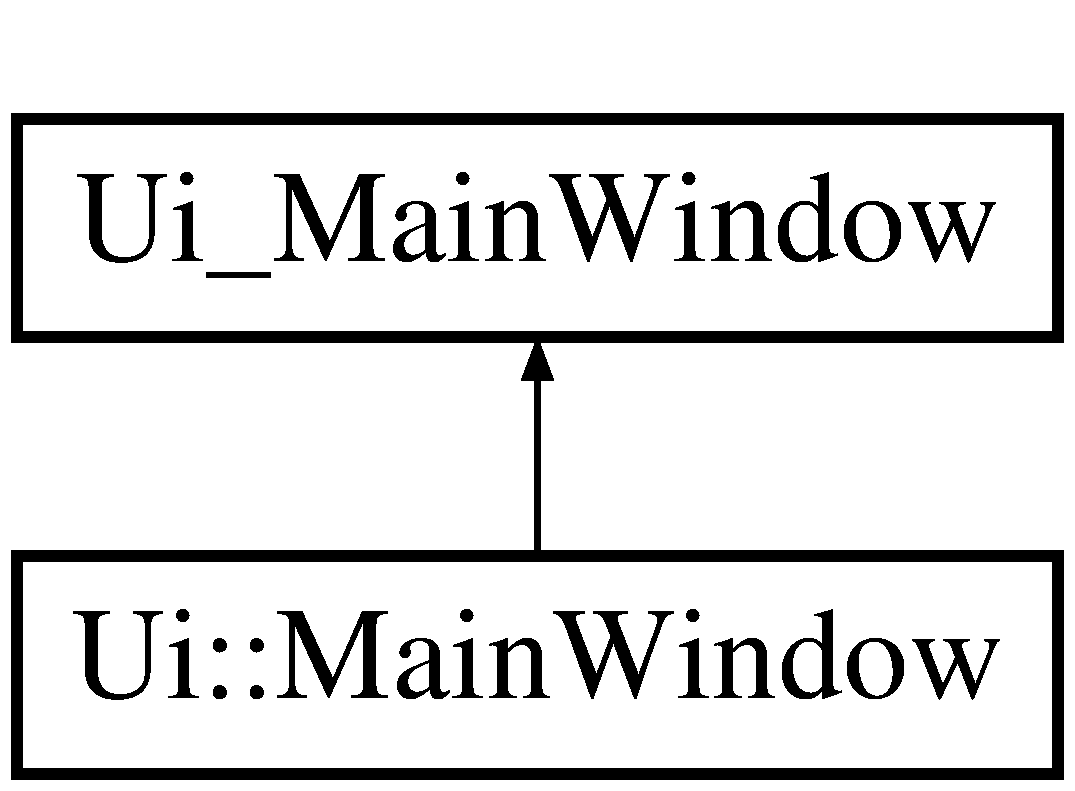
\includegraphics[height=2.000000cm]{class_ui___main_window}
\end{center}
\end{figure}
\subsection*{Public Member Functions}
\begin{DoxyCompactItemize}
\item 
void \mbox{\hyperlink{class_ui___main_window_acf4a0872c4c77d8f43a2ec66ed849b58}{setup\+Ui}} (Q\+Main\+Window $\ast$\mbox{\hyperlink{class_main_window}{Main\+Window}})
\item 
void \mbox{\hyperlink{class_ui___main_window_a097dd160c3534a204904cb374412c618}{retranslate\+Ui}} (Q\+Main\+Window $\ast$\mbox{\hyperlink{class_main_window}{Main\+Window}})
\end{DoxyCompactItemize}
\subsection*{Public Attributes}
\begin{DoxyCompactItemize}
\item 
Q\+Widget $\ast$ \mbox{\hyperlink{class_ui___main_window_a30075506c2116c3ed4ff25e07ae75f81}{central\+Widget}}
\item 
Q\+H\+Box\+Layout $\ast$ \mbox{\hyperlink{class_ui___main_window_a03ce63974cc69b067c91bbf285cceca8}{horizontal\+Layout\+\_\+3}}
\item 
Q\+Group\+Box $\ast$ \mbox{\hyperlink{class_ui___main_window_aef7cb3be8cecfc9aaf98f036a98781ce}{group\+Box}}
\item 
Q\+H\+Box\+Layout $\ast$ \mbox{\hyperlink{class_ui___main_window_acd6fdc9ebacc4b25b834162380d75ce8}{horizontal\+Layout}}
\item 
Q\+List\+Widget $\ast$ \mbox{\hyperlink{class_ui___main_window_ae647a15635ba8a0e5d5aec475db99d8f}{list\+Widget}}
\item 
Q\+Group\+Box $\ast$ \mbox{\hyperlink{class_ui___main_window_abb28acde35ffce4d0e6152579df2cbc3}{group\+Box\+\_\+2}}
\item 
Q\+H\+Box\+Layout $\ast$ \mbox{\hyperlink{class_ui___main_window_a80867018070156432923d0266cc9fe25}{horizontal\+Layout\+\_\+2}}
\item 
Q\+Text\+Browser $\ast$ \mbox{\hyperlink{class_ui___main_window_a2c789c07fa5fc1cee05aae8df52bb02d}{text\+Browser}}
\item 
Q\+Menu\+Bar $\ast$ \mbox{\hyperlink{class_ui___main_window_a2be1c24ec9adfca18e1dcc951931457f}{menu\+Bar}}
\item 
Q\+Tool\+Bar $\ast$ \mbox{\hyperlink{class_ui___main_window_a5172877001c8c7b4e0f6de50421867d1}{main\+Tool\+Bar}}
\item 
Q\+Status\+Bar $\ast$ \mbox{\hyperlink{class_ui___main_window_a50fa481337604bcc8bf68de18ab16ecd}{status\+Bar}}
\end{DoxyCompactItemize}


\subsection{Member Function Documentation}
\mbox{\Hypertarget{class_ui___main_window_a097dd160c3534a204904cb374412c618}\label{class_ui___main_window_a097dd160c3534a204904cb374412c618}} 
\index{Ui\+\_\+\+Main\+Window@{Ui\+\_\+\+Main\+Window}!retranslate\+Ui@{retranslate\+Ui}}
\index{retranslate\+Ui@{retranslate\+Ui}!Ui\+\_\+\+Main\+Window@{Ui\+\_\+\+Main\+Window}}
\subsubsection{\texorpdfstring{retranslate\+Ui()}{retranslateUi()}}
{\footnotesize\ttfamily void Ui\+\_\+\+Main\+Window\+::retranslate\+Ui (\begin{DoxyParamCaption}\item[{Q\+Main\+Window $\ast$}]{Main\+Window }\end{DoxyParamCaption})\hspace{0.3cm}{\ttfamily [inline]}}

\mbox{\Hypertarget{class_ui___main_window_acf4a0872c4c77d8f43a2ec66ed849b58}\label{class_ui___main_window_acf4a0872c4c77d8f43a2ec66ed849b58}} 
\index{Ui\+\_\+\+Main\+Window@{Ui\+\_\+\+Main\+Window}!setup\+Ui@{setup\+Ui}}
\index{setup\+Ui@{setup\+Ui}!Ui\+\_\+\+Main\+Window@{Ui\+\_\+\+Main\+Window}}
\subsubsection{\texorpdfstring{setup\+Ui()}{setupUi()}}
{\footnotesize\ttfamily void Ui\+\_\+\+Main\+Window\+::setup\+Ui (\begin{DoxyParamCaption}\item[{Q\+Main\+Window $\ast$}]{Main\+Window }\end{DoxyParamCaption})\hspace{0.3cm}{\ttfamily [inline]}}



\subsection{Member Data Documentation}
\mbox{\Hypertarget{class_ui___main_window_a30075506c2116c3ed4ff25e07ae75f81}\label{class_ui___main_window_a30075506c2116c3ed4ff25e07ae75f81}} 
\index{Ui\+\_\+\+Main\+Window@{Ui\+\_\+\+Main\+Window}!central\+Widget@{central\+Widget}}
\index{central\+Widget@{central\+Widget}!Ui\+\_\+\+Main\+Window@{Ui\+\_\+\+Main\+Window}}
\subsubsection{\texorpdfstring{central\+Widget}{centralWidget}}
{\footnotesize\ttfamily Q\+Widget$\ast$ Ui\+\_\+\+Main\+Window\+::central\+Widget}

\mbox{\Hypertarget{class_ui___main_window_aef7cb3be8cecfc9aaf98f036a98781ce}\label{class_ui___main_window_aef7cb3be8cecfc9aaf98f036a98781ce}} 
\index{Ui\+\_\+\+Main\+Window@{Ui\+\_\+\+Main\+Window}!group\+Box@{group\+Box}}
\index{group\+Box@{group\+Box}!Ui\+\_\+\+Main\+Window@{Ui\+\_\+\+Main\+Window}}
\subsubsection{\texorpdfstring{group\+Box}{groupBox}}
{\footnotesize\ttfamily Q\+Group\+Box$\ast$ Ui\+\_\+\+Main\+Window\+::group\+Box}

\mbox{\Hypertarget{class_ui___main_window_abb28acde35ffce4d0e6152579df2cbc3}\label{class_ui___main_window_abb28acde35ffce4d0e6152579df2cbc3}} 
\index{Ui\+\_\+\+Main\+Window@{Ui\+\_\+\+Main\+Window}!group\+Box\+\_\+2@{group\+Box\+\_\+2}}
\index{group\+Box\+\_\+2@{group\+Box\+\_\+2}!Ui\+\_\+\+Main\+Window@{Ui\+\_\+\+Main\+Window}}
\subsubsection{\texorpdfstring{group\+Box\+\_\+2}{groupBox\_2}}
{\footnotesize\ttfamily Q\+Group\+Box$\ast$ Ui\+\_\+\+Main\+Window\+::group\+Box\+\_\+2}

\mbox{\Hypertarget{class_ui___main_window_acd6fdc9ebacc4b25b834162380d75ce8}\label{class_ui___main_window_acd6fdc9ebacc4b25b834162380d75ce8}} 
\index{Ui\+\_\+\+Main\+Window@{Ui\+\_\+\+Main\+Window}!horizontal\+Layout@{horizontal\+Layout}}
\index{horizontal\+Layout@{horizontal\+Layout}!Ui\+\_\+\+Main\+Window@{Ui\+\_\+\+Main\+Window}}
\subsubsection{\texorpdfstring{horizontal\+Layout}{horizontalLayout}}
{\footnotesize\ttfamily Q\+H\+Box\+Layout$\ast$ Ui\+\_\+\+Main\+Window\+::horizontal\+Layout}

\mbox{\Hypertarget{class_ui___main_window_a80867018070156432923d0266cc9fe25}\label{class_ui___main_window_a80867018070156432923d0266cc9fe25}} 
\index{Ui\+\_\+\+Main\+Window@{Ui\+\_\+\+Main\+Window}!horizontal\+Layout\+\_\+2@{horizontal\+Layout\+\_\+2}}
\index{horizontal\+Layout\+\_\+2@{horizontal\+Layout\+\_\+2}!Ui\+\_\+\+Main\+Window@{Ui\+\_\+\+Main\+Window}}
\subsubsection{\texorpdfstring{horizontal\+Layout\+\_\+2}{horizontalLayout\_2}}
{\footnotesize\ttfamily Q\+H\+Box\+Layout$\ast$ Ui\+\_\+\+Main\+Window\+::horizontal\+Layout\+\_\+2}

\mbox{\Hypertarget{class_ui___main_window_a03ce63974cc69b067c91bbf285cceca8}\label{class_ui___main_window_a03ce63974cc69b067c91bbf285cceca8}} 
\index{Ui\+\_\+\+Main\+Window@{Ui\+\_\+\+Main\+Window}!horizontal\+Layout\+\_\+3@{horizontal\+Layout\+\_\+3}}
\index{horizontal\+Layout\+\_\+3@{horizontal\+Layout\+\_\+3}!Ui\+\_\+\+Main\+Window@{Ui\+\_\+\+Main\+Window}}
\subsubsection{\texorpdfstring{horizontal\+Layout\+\_\+3}{horizontalLayout\_3}}
{\footnotesize\ttfamily Q\+H\+Box\+Layout$\ast$ Ui\+\_\+\+Main\+Window\+::horizontal\+Layout\+\_\+3}

\mbox{\Hypertarget{class_ui___main_window_ae647a15635ba8a0e5d5aec475db99d8f}\label{class_ui___main_window_ae647a15635ba8a0e5d5aec475db99d8f}} 
\index{Ui\+\_\+\+Main\+Window@{Ui\+\_\+\+Main\+Window}!list\+Widget@{list\+Widget}}
\index{list\+Widget@{list\+Widget}!Ui\+\_\+\+Main\+Window@{Ui\+\_\+\+Main\+Window}}
\subsubsection{\texorpdfstring{list\+Widget}{listWidget}}
{\footnotesize\ttfamily Q\+List\+Widget$\ast$ Ui\+\_\+\+Main\+Window\+::list\+Widget}

\mbox{\Hypertarget{class_ui___main_window_a5172877001c8c7b4e0f6de50421867d1}\label{class_ui___main_window_a5172877001c8c7b4e0f6de50421867d1}} 
\index{Ui\+\_\+\+Main\+Window@{Ui\+\_\+\+Main\+Window}!main\+Tool\+Bar@{main\+Tool\+Bar}}
\index{main\+Tool\+Bar@{main\+Tool\+Bar}!Ui\+\_\+\+Main\+Window@{Ui\+\_\+\+Main\+Window}}
\subsubsection{\texorpdfstring{main\+Tool\+Bar}{mainToolBar}}
{\footnotesize\ttfamily Q\+Tool\+Bar$\ast$ Ui\+\_\+\+Main\+Window\+::main\+Tool\+Bar}

\mbox{\Hypertarget{class_ui___main_window_a2be1c24ec9adfca18e1dcc951931457f}\label{class_ui___main_window_a2be1c24ec9adfca18e1dcc951931457f}} 
\index{Ui\+\_\+\+Main\+Window@{Ui\+\_\+\+Main\+Window}!menu\+Bar@{menu\+Bar}}
\index{menu\+Bar@{menu\+Bar}!Ui\+\_\+\+Main\+Window@{Ui\+\_\+\+Main\+Window}}
\subsubsection{\texorpdfstring{menu\+Bar}{menuBar}}
{\footnotesize\ttfamily Q\+Menu\+Bar$\ast$ Ui\+\_\+\+Main\+Window\+::menu\+Bar}

\mbox{\Hypertarget{class_ui___main_window_a50fa481337604bcc8bf68de18ab16ecd}\label{class_ui___main_window_a50fa481337604bcc8bf68de18ab16ecd}} 
\index{Ui\+\_\+\+Main\+Window@{Ui\+\_\+\+Main\+Window}!status\+Bar@{status\+Bar}}
\index{status\+Bar@{status\+Bar}!Ui\+\_\+\+Main\+Window@{Ui\+\_\+\+Main\+Window}}
\subsubsection{\texorpdfstring{status\+Bar}{statusBar}}
{\footnotesize\ttfamily Q\+Status\+Bar$\ast$ Ui\+\_\+\+Main\+Window\+::status\+Bar}

\mbox{\Hypertarget{class_ui___main_window_a2c789c07fa5fc1cee05aae8df52bb02d}\label{class_ui___main_window_a2c789c07fa5fc1cee05aae8df52bb02d}} 
\index{Ui\+\_\+\+Main\+Window@{Ui\+\_\+\+Main\+Window}!text\+Browser@{text\+Browser}}
\index{text\+Browser@{text\+Browser}!Ui\+\_\+\+Main\+Window@{Ui\+\_\+\+Main\+Window}}
\subsubsection{\texorpdfstring{text\+Browser}{textBrowser}}
{\footnotesize\ttfamily Q\+Text\+Browser$\ast$ Ui\+\_\+\+Main\+Window\+::text\+Browser}



The documentation for this class was generated from the following file\+:\begin{DoxyCompactItemize}
\item 
\mbox{\hyperlink{ui__mainwindow_8h}{ui\+\_\+mainwindow.\+h}}\end{DoxyCompactItemize}

\chapter{File Documentation}
\hypertarget{datastorage_8cpp}{}\section{datastorage.\+cpp File Reference}
\label{datastorage_8cpp}\index{datastorage.\+cpp@{datastorage.\+cpp}}
{\ttfamily \#include \char`\"{}datastorage.\+h\char`\"{}}\newline
{\ttfamily \#include $<$Q\+Mutex\+Locker$>$}\newline
{\ttfamily \#include $<$Q\+Debug$>$}\newline
\subsection*{Classes}
\begin{DoxyCompactItemize}
\item 
struct \mbox{\hyperlink{struct_range_test}{Range\+Test}}
\end{DoxyCompactItemize}

\hypertarget{datastorage_8h}{}\section{datastorage.\+h File Reference}
\label{datastorage_8h}\index{datastorage.\+h@{datastorage.\+h}}
{\ttfamily \#include $<$Q\+Date\+Time$>$}\newline
{\ttfamily \#include $<$Q\+Host\+Address$>$}\newline
{\ttfamily \#include $<$Q\+Mutex$>$}\newline
{\ttfamily \#include $<$Q\+Map$>$}\newline
{\ttfamily \#include $<$vector$>$}\newline
\subsection*{Classes}
\begin{DoxyCompactItemize}
\item 
struct \mbox{\hyperlink{struct_entry}{Entry}}
\item 
class \mbox{\hyperlink{class_data_storage}{Data\+Storage}}
\end{DoxyCompactItemize}

\hypertarget{main_8cpp}{}\section{main.\+cpp File Reference}
\label{main_8cpp}\index{main.\+cpp@{main.\+cpp}}
{\ttfamily \#include $<$iostream$>$}\newline
{\ttfamily \#include $<$vector$>$}\newline
{\ttfamily \#include \char`\"{}figurageometrica.\+h\char`\"{}}\newline
{\ttfamily \#include \char`\"{}reta.\+h\char`\"{}}\newline
{\ttfamily \#include \char`\"{}retangulo.\+h\char`\"{}}\newline
{\ttfamily \#include \char`\"{}circulo.\+h\char`\"{}}\newline
{\ttfamily \#include \char`\"{}ponto.\+h\char`\"{}}\newline
{\ttfamily \#include \char`\"{}screen.\+h\char`\"{}}\newline
{\ttfamily \#include $<$fstream$>$}\newline
\subsection*{Functions}
\begin{DoxyCompactItemize}
\item 
int \mbox{\hyperlink{main_8cpp_ae66f6b31b5ad750f1fe042a706a4e3d4}{main}} ()
\end{DoxyCompactItemize}


\subsection{Function Documentation}
\mbox{\Hypertarget{main_8cpp_ae66f6b31b5ad750f1fe042a706a4e3d4}\label{main_8cpp_ae66f6b31b5ad750f1fe042a706a4e3d4}} 
\index{main.\+cpp@{main.\+cpp}!main@{main}}
\index{main@{main}!main.\+cpp@{main.\+cpp}}
\subsubsection{\texorpdfstring{main()}{main()}}
{\footnotesize\ttfamily int main (\begin{DoxyParamCaption}{ }\end{DoxyParamCaption})}


\hypertarget{mainwindow_8cpp}{}\section{mainwindow.\+cpp File Reference}
\label{mainwindow_8cpp}\index{mainwindow.\+cpp@{mainwindow.\+cpp}}
{\ttfamily \#include \char`\"{}mainwindow.\+h\char`\"{}}\newline
{\ttfamily \#include \char`\"{}ui\+\_\+mainwindow.\+h\char`\"{}}\newline
{\ttfamily \#include \char`\"{}myserver.\+h\char`\"{}}\newline
{\ttfamily \#include $<$Q\+String\+List$>$}\newline

\hypertarget{mainwindow_8h}{}\section{mainwindow.\+h File Reference}
\label{mainwindow_8h}\index{mainwindow.\+h@{mainwindow.\+h}}
{\ttfamily \#include $<$Q\+Main\+Window$>$}\newline
{\ttfamily \#include $<$Q\+Tcp\+Socket$>$}\newline
{\ttfamily \#include $<$Q\+Debug$>$}\newline
{\ttfamily \#include $<$Q\+Timer$>$}\newline
\subsection*{Classes}
\begin{DoxyCompactItemize}
\item 
class \mbox{\hyperlink{class_main_window}{Main\+Window}}
\begin{DoxyCompactList}\small\item\em The \mbox{\hyperlink{class_main_window}{Main\+Window}} class Classe da janela principal do consumidor de dados. \end{DoxyCompactList}\end{DoxyCompactItemize}
\subsection*{Namespaces}
\begin{DoxyCompactItemize}
\item 
 \mbox{\hyperlink{namespace_ui}{Ui}}
\end{DoxyCompactItemize}

\hypertarget{moc__mainwindow_8cpp}{}\section{moc\+\_\+mainwindow.\+cpp File Reference}
\label{moc__mainwindow_8cpp}\index{moc\+\_\+mainwindow.\+cpp@{moc\+\_\+mainwindow.\+cpp}}
{\ttfamily \#include \char`\"{}mainwindow.\+h\char`\"{}}\newline
{\ttfamily \#include $<$Qt\+Core/qbytearray.\+h$>$}\newline
{\ttfamily \#include $<$Qt\+Core/qmetatype.\+h$>$}\newline
\subsection*{Classes}
\begin{DoxyCompactItemize}
\item 
struct \mbox{\hyperlink{structqt__meta__stringdata___main_window__t}{qt\+\_\+meta\+\_\+stringdata\+\_\+\+Main\+Window\+\_\+t}}
\end{DoxyCompactItemize}
\subsection*{Macros}
\begin{DoxyCompactItemize}
\item 
\#define \mbox{\hyperlink{moc__mainwindow_8cpp_a75bb9482d242cde0a06c9dbdc6b83abe}{Q\+T\+\_\+\+M\+O\+C\+\_\+\+L\+I\+T\+E\+R\+AL}}(idx,  ofs,  len)
\end{DoxyCompactItemize}


\subsection{Macro Definition Documentation}
\mbox{\Hypertarget{moc__mainwindow_8cpp_a75bb9482d242cde0a06c9dbdc6b83abe}\label{moc__mainwindow_8cpp_a75bb9482d242cde0a06c9dbdc6b83abe}} 
\index{moc\+\_\+mainwindow.\+cpp@{moc\+\_\+mainwindow.\+cpp}!Q\+T\+\_\+\+M\+O\+C\+\_\+\+L\+I\+T\+E\+R\+AL@{Q\+T\+\_\+\+M\+O\+C\+\_\+\+L\+I\+T\+E\+R\+AL}}
\index{Q\+T\+\_\+\+M\+O\+C\+\_\+\+L\+I\+T\+E\+R\+AL@{Q\+T\+\_\+\+M\+O\+C\+\_\+\+L\+I\+T\+E\+R\+AL}!moc\+\_\+mainwindow.\+cpp@{moc\+\_\+mainwindow.\+cpp}}
\subsubsection{\texorpdfstring{Q\+T\+\_\+\+M\+O\+C\+\_\+\+L\+I\+T\+E\+R\+AL}{QT\_MOC\_LITERAL}}
{\footnotesize\ttfamily \#define Q\+T\+\_\+\+M\+O\+C\+\_\+\+L\+I\+T\+E\+R\+AL(\begin{DoxyParamCaption}\item[{}]{idx,  }\item[{}]{ofs,  }\item[{}]{len }\end{DoxyParamCaption})}

{\bfseries Value\+:}
\begin{DoxyCode}
Q\_STATIC\_BYTE\_ARRAY\_DATA\_HEADER\_INITIALIZER\_WITH\_OFFSET(len, \(\backslash\)
    qptrdiff(offsetof(\mbox{\hyperlink{structqt__meta__stringdata___main_window__t}{qt\_meta\_stringdata\_MainWindow\_t}}, stringdata0) + ofs \(\backslash\)
        - idx * \textcolor{keyword}{sizeof}(QByteArrayData)) \(\backslash\)
    )
\end{DoxyCode}

\hypertarget{moc__myserver_8cpp}{}\section{moc\+\_\+myserver.\+cpp File Reference}
\label{moc__myserver_8cpp}\index{moc\+\_\+myserver.\+cpp@{moc\+\_\+myserver.\+cpp}}
{\ttfamily \#include \char`\"{}myserver.\+h\char`\"{}}\newline
{\ttfamily \#include $<$Qt\+Core/qbytearray.\+h$>$}\newline
{\ttfamily \#include $<$Qt\+Core/qmetatype.\+h$>$}\newline
\subsection*{Classes}
\begin{DoxyCompactItemize}
\item 
struct \mbox{\hyperlink{structqt__meta__stringdata___my_server__t}{qt\+\_\+meta\+\_\+stringdata\+\_\+\+My\+Server\+\_\+t}}
\end{DoxyCompactItemize}
\subsection*{Macros}
\begin{DoxyCompactItemize}
\item 
\#define \mbox{\hyperlink{moc__myserver_8cpp_a75bb9482d242cde0a06c9dbdc6b83abe}{Q\+T\+\_\+\+M\+O\+C\+\_\+\+L\+I\+T\+E\+R\+AL}}(idx,  ofs,  len)
\end{DoxyCompactItemize}


\subsection{Macro Definition Documentation}
\mbox{\Hypertarget{moc__myserver_8cpp_a75bb9482d242cde0a06c9dbdc6b83abe}\label{moc__myserver_8cpp_a75bb9482d242cde0a06c9dbdc6b83abe}} 
\index{moc\+\_\+myserver.\+cpp@{moc\+\_\+myserver.\+cpp}!Q\+T\+\_\+\+M\+O\+C\+\_\+\+L\+I\+T\+E\+R\+AL@{Q\+T\+\_\+\+M\+O\+C\+\_\+\+L\+I\+T\+E\+R\+AL}}
\index{Q\+T\+\_\+\+M\+O\+C\+\_\+\+L\+I\+T\+E\+R\+AL@{Q\+T\+\_\+\+M\+O\+C\+\_\+\+L\+I\+T\+E\+R\+AL}!moc\+\_\+myserver.\+cpp@{moc\+\_\+myserver.\+cpp}}
\subsubsection{\texorpdfstring{Q\+T\+\_\+\+M\+O\+C\+\_\+\+L\+I\+T\+E\+R\+AL}{QT\_MOC\_LITERAL}}
{\footnotesize\ttfamily \#define Q\+T\+\_\+\+M\+O\+C\+\_\+\+L\+I\+T\+E\+R\+AL(\begin{DoxyParamCaption}\item[{}]{idx,  }\item[{}]{ofs,  }\item[{}]{len }\end{DoxyParamCaption})}

{\bfseries Value\+:}
\begin{DoxyCode}
Q\_STATIC\_BYTE\_ARRAY\_DATA\_HEADER\_INITIALIZER\_WITH\_OFFSET(len, \(\backslash\)
    qptrdiff(offsetof(\mbox{\hyperlink{structqt__meta__stringdata___my_server__t}{qt\_meta\_stringdata\_MyServer\_t}}, stringdata0) + ofs \(\backslash\)
        - idx * \textcolor{keyword}{sizeof}(QByteArrayData)) \(\backslash\)
    )
\end{DoxyCode}

\hypertarget{moc__mythread_8cpp}{}\section{moc\+\_\+mythread.\+cpp File Reference}
\label{moc__mythread_8cpp}\index{moc\+\_\+mythread.\+cpp@{moc\+\_\+mythread.\+cpp}}
{\ttfamily \#include \char`\"{}mythread.\+h\char`\"{}}\newline
{\ttfamily \#include $<$Qt\+Core/qbytearray.\+h$>$}\newline
{\ttfamily \#include $<$Qt\+Core/qmetatype.\+h$>$}\newline
\subsection*{Classes}
\begin{DoxyCompactItemize}
\item 
struct \mbox{\hyperlink{structqt__meta__stringdata___my_thread__t}{qt\+\_\+meta\+\_\+stringdata\+\_\+\+My\+Thread\+\_\+t}}
\end{DoxyCompactItemize}
\subsection*{Macros}
\begin{DoxyCompactItemize}
\item 
\#define \mbox{\hyperlink{moc__mythread_8cpp_a75bb9482d242cde0a06c9dbdc6b83abe}{Q\+T\+\_\+\+M\+O\+C\+\_\+\+L\+I\+T\+E\+R\+AL}}(idx,  ofs,  len)
\end{DoxyCompactItemize}


\subsection{Macro Definition Documentation}
\mbox{\Hypertarget{moc__mythread_8cpp_a75bb9482d242cde0a06c9dbdc6b83abe}\label{moc__mythread_8cpp_a75bb9482d242cde0a06c9dbdc6b83abe}} 
\index{moc\+\_\+mythread.\+cpp@{moc\+\_\+mythread.\+cpp}!Q\+T\+\_\+\+M\+O\+C\+\_\+\+L\+I\+T\+E\+R\+AL@{Q\+T\+\_\+\+M\+O\+C\+\_\+\+L\+I\+T\+E\+R\+AL}}
\index{Q\+T\+\_\+\+M\+O\+C\+\_\+\+L\+I\+T\+E\+R\+AL@{Q\+T\+\_\+\+M\+O\+C\+\_\+\+L\+I\+T\+E\+R\+AL}!moc\+\_\+mythread.\+cpp@{moc\+\_\+mythread.\+cpp}}
\subsubsection{\texorpdfstring{Q\+T\+\_\+\+M\+O\+C\+\_\+\+L\+I\+T\+E\+R\+AL}{QT\_MOC\_LITERAL}}
{\footnotesize\ttfamily \#define Q\+T\+\_\+\+M\+O\+C\+\_\+\+L\+I\+T\+E\+R\+AL(\begin{DoxyParamCaption}\item[{}]{idx,  }\item[{}]{ofs,  }\item[{}]{len }\end{DoxyParamCaption})}

{\bfseries Value\+:}
\begin{DoxyCode}
Q\_STATIC\_BYTE\_ARRAY\_DATA\_HEADER\_INITIALIZER\_WITH\_OFFSET(len, \(\backslash\)
    qptrdiff(offsetof(\mbox{\hyperlink{structqt__meta__stringdata___my_thread__t}{qt\_meta\_stringdata\_MyThread\_t}}, stringdata0) + ofs \(\backslash\)
        - idx * \textcolor{keyword}{sizeof}(QByteArrayData)) \(\backslash\)
    )
\end{DoxyCode}

\hypertarget{myserver_8cpp}{}\section{myserver.\+cpp File Reference}
\label{myserver_8cpp}\index{myserver.\+cpp@{myserver.\+cpp}}
{\ttfamily \#include \char`\"{}myserver.\+h\char`\"{}}\newline
{\ttfamily \#include $<$Q\+Network\+Interface$>$}\newline

\hypertarget{myserver_8h}{}\section{myserver.\+h File Reference}
\label{myserver_8h}\index{myserver.\+h@{myserver.\+h}}
{\ttfamily \#include $<$Q\+Tcp\+Server$>$}\newline
{\ttfamily \#include $<$Q\+Debug$>$}\newline
{\ttfamily \#include $<$Q\+String\+List$>$}\newline
{\ttfamily \#include \char`\"{}mythread.\+h\char`\"{}}\newline
{\ttfamily \#include \char`\"{}datastorage.\+h\char`\"{}}\newline
\subsection*{Classes}
\begin{DoxyCompactItemize}
\item 
class \mbox{\hyperlink{class_my_server}{My\+Server}}
\begin{DoxyCompactList}\small\item\em The \mbox{\hyperlink{class_my_server}{My\+Server}} class inicia um servidor T\+CP capaz de \char`\"{}ouvir\char`\"{} a porta 1234. \end{DoxyCompactList}\end{DoxyCompactItemize}

\hypertarget{mythread_8cpp}{}\section{mythread.\+cpp File Reference}
\label{mythread_8cpp}\index{mythread.\+cpp@{mythread.\+cpp}}
{\ttfamily \#include \char`\"{}mythread.\+h\char`\"{}}\newline
{\ttfamily \#include $<$vector$>$}\newline

\hypertarget{mythread_8h}{}\section{mythread.\+h File Reference}
\label{mythread_8h}\index{mythread.\+h@{mythread.\+h}}
{\ttfamily \#include $<$Q\+Object$>$}\newline
{\ttfamily \#include $<$Q\+Thread$>$}\newline
{\ttfamily \#include $<$Q\+Tcp\+Socket$>$}\newline
{\ttfamily \#include $<$Q\+Debug$>$}\newline
{\ttfamily \#include $<$Q\+String\+List$>$}\newline
{\ttfamily \#include $<$Q\+String$>$}\newline
{\ttfamily \#include $<$Q\+Host\+Address$>$}\newline
{\ttfamily \#include \char`\"{}datastorage.\+h\char`\"{}}\newline
\subsection*{Classes}
\begin{DoxyCompactItemize}
\item 
class \mbox{\hyperlink{class_my_thread}{My\+Thread}}
\begin{DoxyCompactList}\small\item\em The \mbox{\hyperlink{class_my_thread}{My\+Thread}} class cria uma thread que lida com o tratamento de uma conexao T\+CP de entrada. \end{DoxyCompactList}\end{DoxyCompactItemize}

\hypertarget{ui__mainwindow_8h}{}\section{ui\+\_\+mainwindow.\+h File Reference}
\label{ui__mainwindow_8h}\index{ui\+\_\+mainwindow.\+h@{ui\+\_\+mainwindow.\+h}}
{\ttfamily \#include $<$Qt\+Core/\+Q\+Variant$>$}\newline
{\ttfamily \#include $<$Qt\+Widgets/\+Q\+Action$>$}\newline
{\ttfamily \#include $<$Qt\+Widgets/\+Q\+Application$>$}\newline
{\ttfamily \#include $<$Qt\+Widgets/\+Q\+Button\+Group$>$}\newline
{\ttfamily \#include $<$Qt\+Widgets/\+Q\+Group\+Box$>$}\newline
{\ttfamily \#include $<$Qt\+Widgets/\+Q\+H\+Box\+Layout$>$}\newline
{\ttfamily \#include $<$Qt\+Widgets/\+Q\+Header\+View$>$}\newline
{\ttfamily \#include $<$Qt\+Widgets/\+Q\+List\+Widget$>$}\newline
{\ttfamily \#include $<$Qt\+Widgets/\+Q\+Main\+Window$>$}\newline
{\ttfamily \#include $<$Qt\+Widgets/\+Q\+Menu\+Bar$>$}\newline
{\ttfamily \#include $<$Qt\+Widgets/\+Q\+Status\+Bar$>$}\newline
{\ttfamily \#include $<$Qt\+Widgets/\+Q\+Text\+Browser$>$}\newline
{\ttfamily \#include $<$Qt\+Widgets/\+Q\+Tool\+Bar$>$}\newline
{\ttfamily \#include $<$Qt\+Widgets/\+Q\+Widget$>$}\newline
\subsection*{Classes}
\begin{DoxyCompactItemize}
\item 
class \mbox{\hyperlink{class_ui___main_window}{Ui\+\_\+\+Main\+Window}}
\item 
class \mbox{\hyperlink{class_ui_1_1_main_window}{Ui\+::\+Main\+Window}}
\end{DoxyCompactItemize}
\subsection*{Namespaces}
\begin{DoxyCompactItemize}
\item 
 \mbox{\hyperlink{namespace_ui}{Ui}}
\end{DoxyCompactItemize}

%--- End generated contents ---

% Index
\backmatter
\newpage
\phantomsection
\clearemptydoublepage
\addcontentsline{toc}{chapter}{Index}
\printindex

\end{document}
